%%%%%%%%%%%%%%%%%%%%%%%%%%%%%%%%%%%%%%%%%
% Simple Sectioned Essay Template
% LaTeX Template
%
% This template has been downloaded from:
% http://www.latextemplates.com
%
% Note:
% The \lipsum[#] commands throughout this template generate dummy text
% to fill the template out. These commands should all be removed when 
% writing essay content.
%
%%%%%%%%%%%%%%%%%%%%%%%%%%%%%%%%%%%%%%%%

%----------------------------------------------------------------------------------------
%	PACKAGES AND OTHER DOCUMENT CONFIGURATIONS
%----------------------------------------------------------------------------------------

\documentclass[12pt]{article} % Default font size is 12pt, it can be changed here

\usepackage{geometry} % Required to change the page size to A4
\geometry{a4paper} % Set the page size to be A4 as opposed to the default US Letter

\usepackage{graphicx} % Required for including pictures
\usepackage{pdfpages}
\usepackage{float} % Allows putting an [H] in \begin{figure} to specify the exact location of the figure
\usepackage{wrapfig} % Allows in-line images such as the example fish picture
\usepackage{float}
\usepackage{lipsum} % Used for inserting dummy 'Lorem ipsum' text into the template

\linespread{1.2} % Line spacing

%\setlength\parindent{0pt} % Uncomment to remove all indentation from paragraphs

\graphicspath{{Pictures/}} % Specifies the directory where pictures are stored

\begin{document}


%----------------------------------------------------------------------------------------
%	TITLE PAGE
%----------------------------------------------------------------------------------------

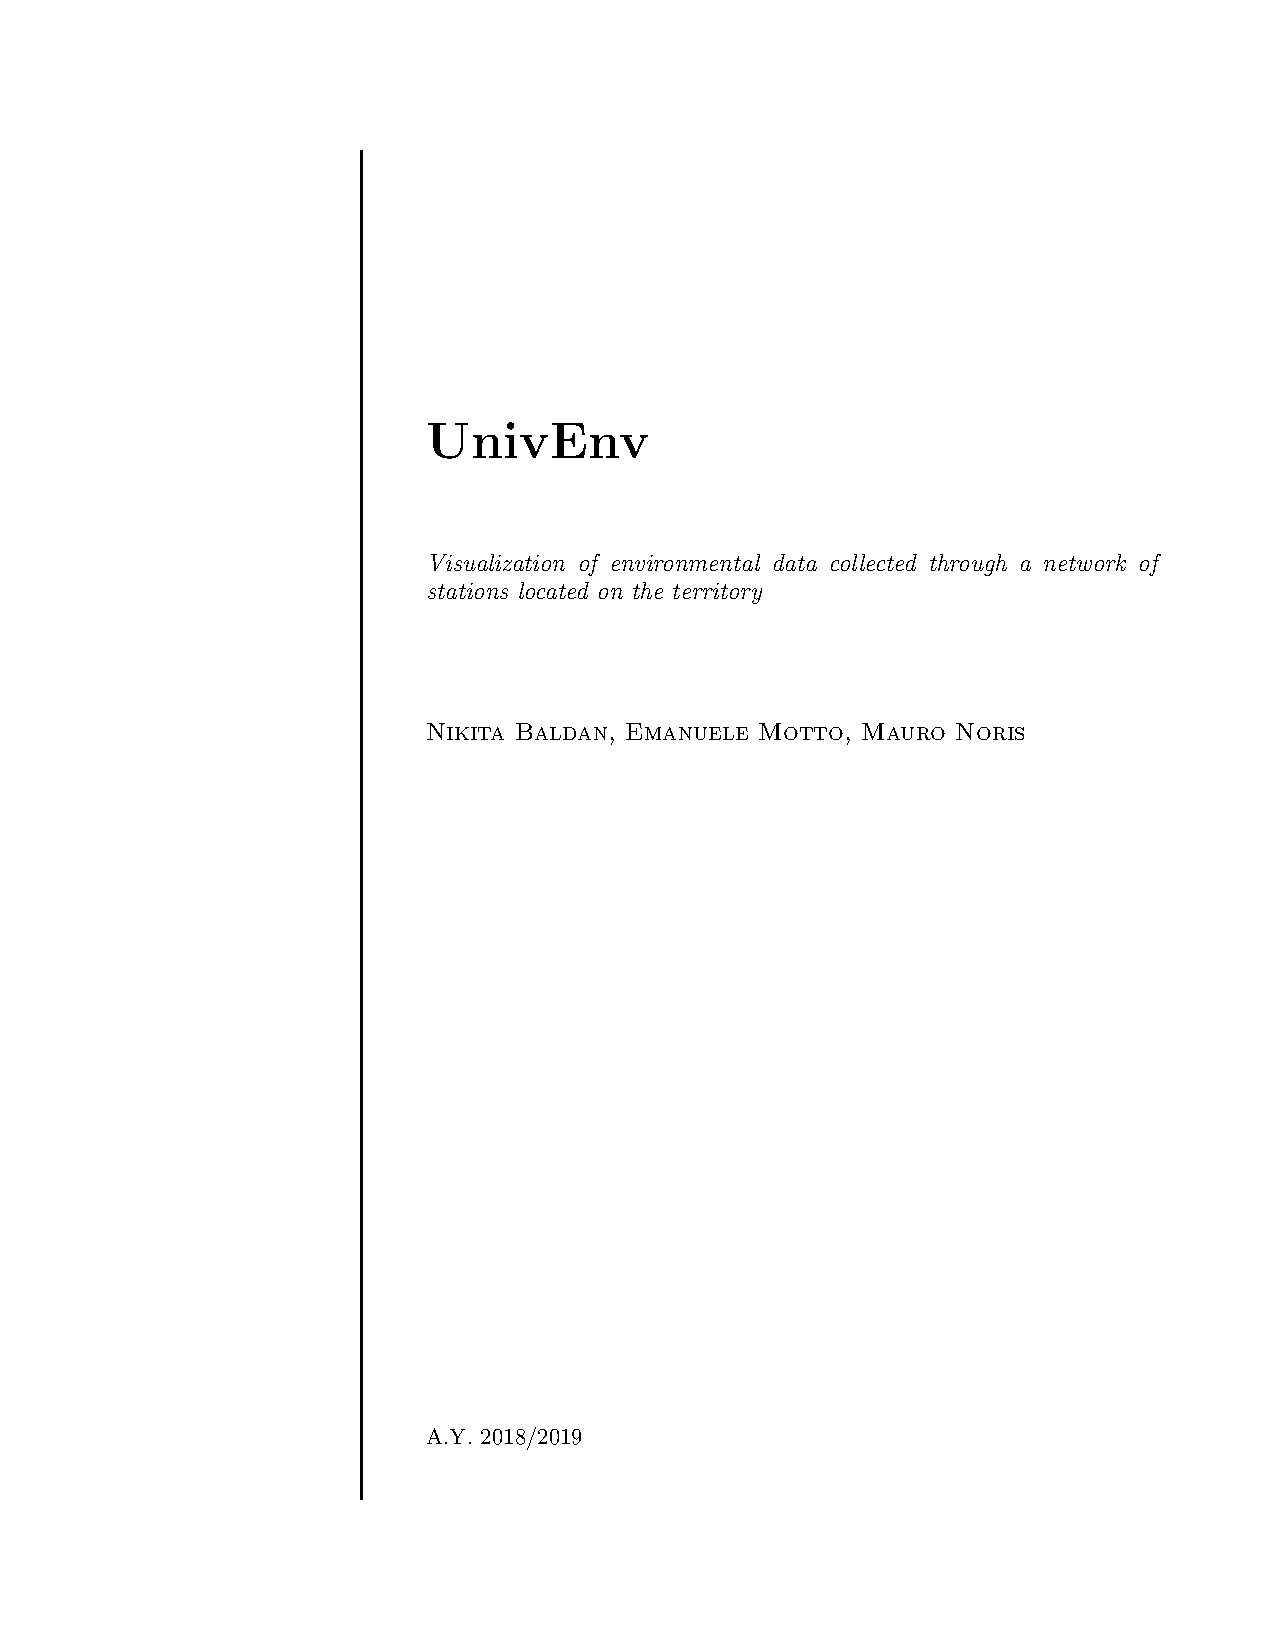
\includepdf[page={1}]{title}
%----------------------------------------------------------------------------------------
%	TABLE OF CONTENTS
%----------------------------------------------------------------------------------------

\tableofcontents % Include a table of contents

\newpage % Begins the essay on a new page instead of on the same page as the table of contents 

%----------------------------------------------------------------------------------------
%	INTRODUCTION
%----------------------------------------------------------------------------------------

\section{Introduction} % Major section
The main topic of this project is to provide a set of visualization tools regarding environmental data collected by a station located in the territory.\\
The requirement is to design three different information visualization tools, which are the following:
\begin{itemize}
\item Individual: app for smartphone/smartwatch
\item Public: ambient display
\item Technical: application for large tablets or desktop
\end{itemize}
Each of the representation is linked by a different type of user, for example the desktop application is made for  letting back end technical personnel  staff to access data at different levels of granularity, instead of the public representation that will provide an approximation of the data collection for letting not technical people understand what they're seeing.\\
\section{Data}
The station will collect the following environmental data:
\begin{itemize}
\item CO2
\item Air Humidity
\item Luminosity
\item Wind speed and direction 
\item Location (also height, type of soil, type of surrounding environment)
\item Time (hour/season)
\item Pressure
\item Rain
\item Temperature
\section{Competitive analisys}
\subsection{Personal interface}
Before we could actualy start the design, a little research on the argument had to be done, about the data representation techniques which could be used with the data we have to visualize and some examples of application which dealed with something similar.

We found some good examples and took some hints.
\subsubsection{Air visual}
This was a good app to start the competitive analysis, because it was the most complete and the prettiest.
We deduced from this app we can organize the general look of the application as a n card view, and there was some historic data management we found vey interesting.
\begin{figure}[H]
  \centering
  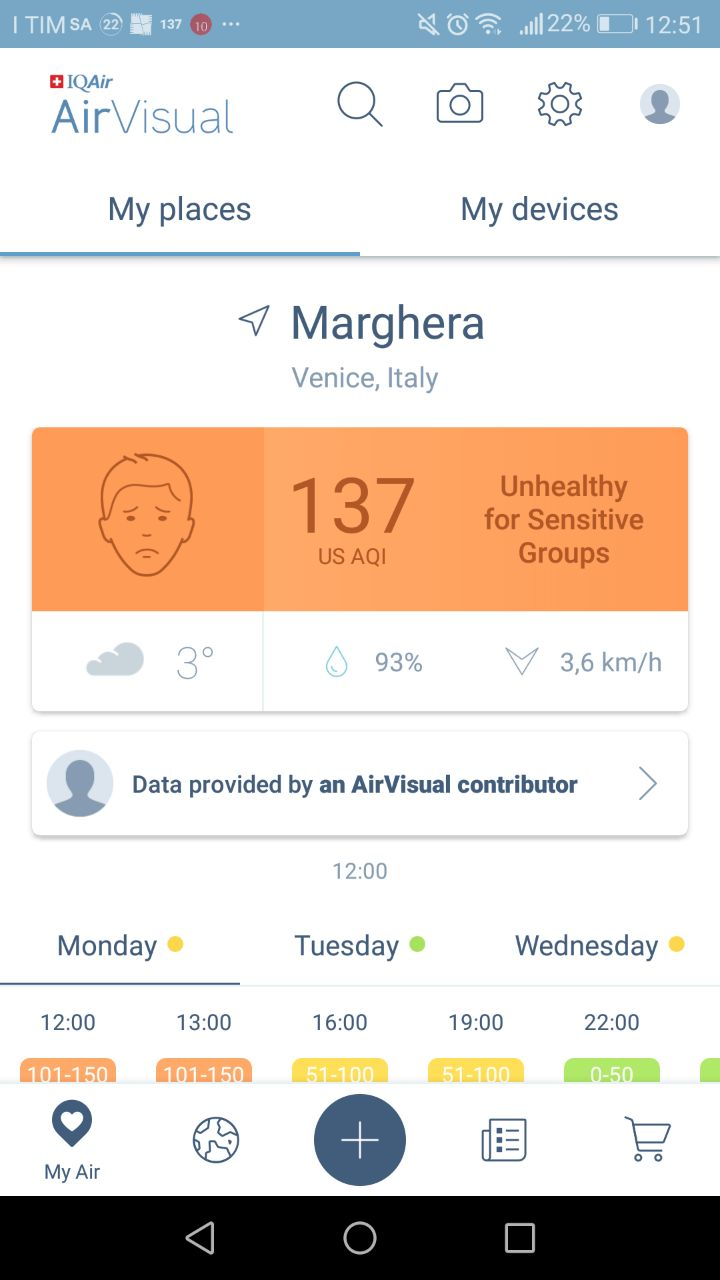
\includegraphics[width=4cm,height=10cm,keepaspectratio]{img/AirVisual1.jpeg}
  \hspace{0.1\textwidth}
  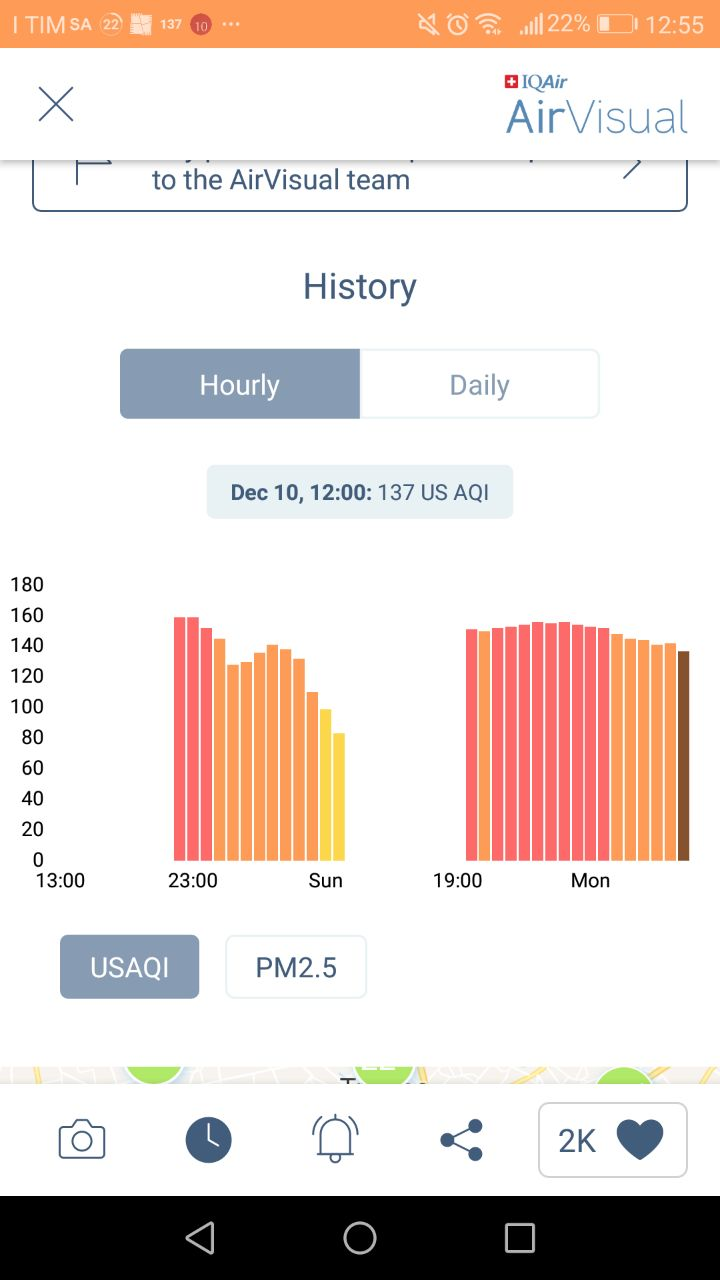
\includegraphics[width=4cm,height=10cm,keepaspectratio]{img/AirVisual2.jpeg}
  \hfill
  \caption{As we can see, the left most img has a 2-card design(My places/My devices), while the right most
  has a daily/hourly historic data.}
  \label{fig:boat4}
\end{figure}


\subsubsection{Air Quality:Real Time AQI}
From this app, we found really interesting the data visualization through histogram diagram and they visualize the data in a certain timespan.
\begin{figure}[H]
  \centering
  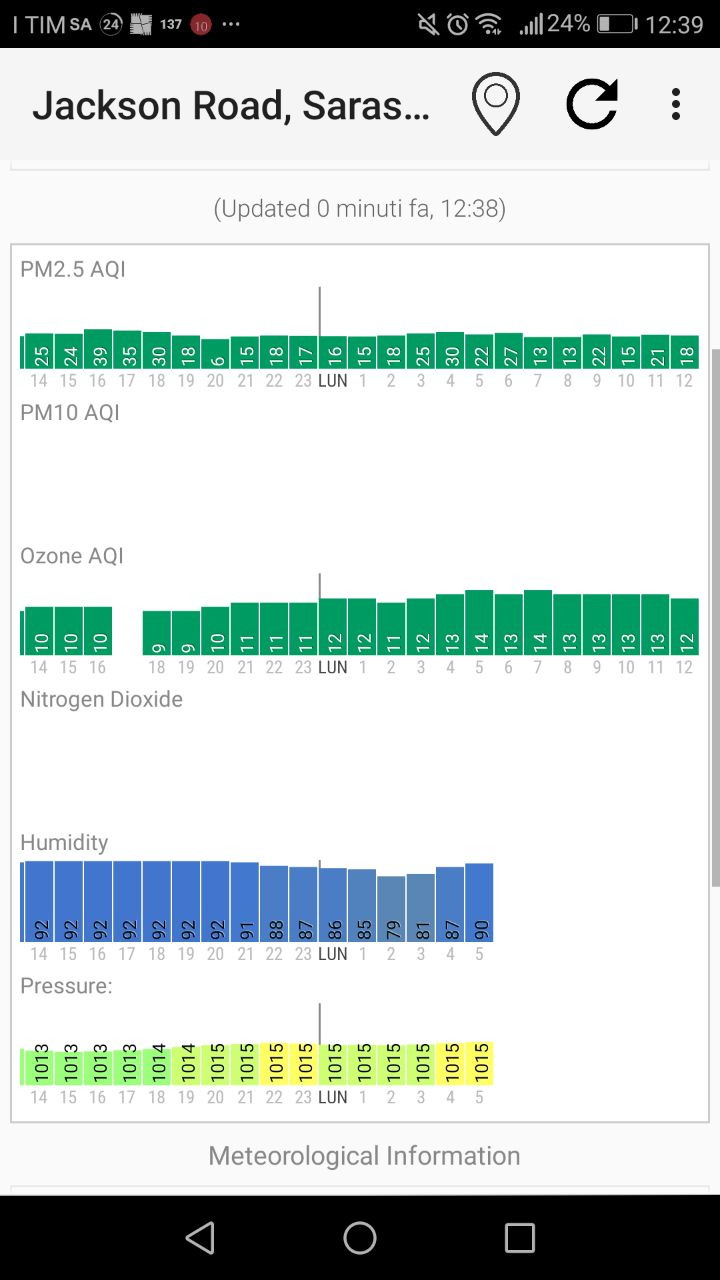
\includegraphics[width=4cm,height=10cm,keepaspectratio]{img/apphistogram.jpeg}
  \caption{Airquality histograms}
  \label{fig:boat3}
\end{figure}

\subsection{Technical Interface}
For the technical we searched for desktop online application and sites which treated the same kind of data(meteorologic, air pollution).

\subsubsection{acqin.org}
The site displays a large map with colored indicators that indicate the quality of the air in zone where the centers are placed. The use of colours permits a good comparison among the various centers.
\begin{figure}[H]
  \centering
  \hfill
  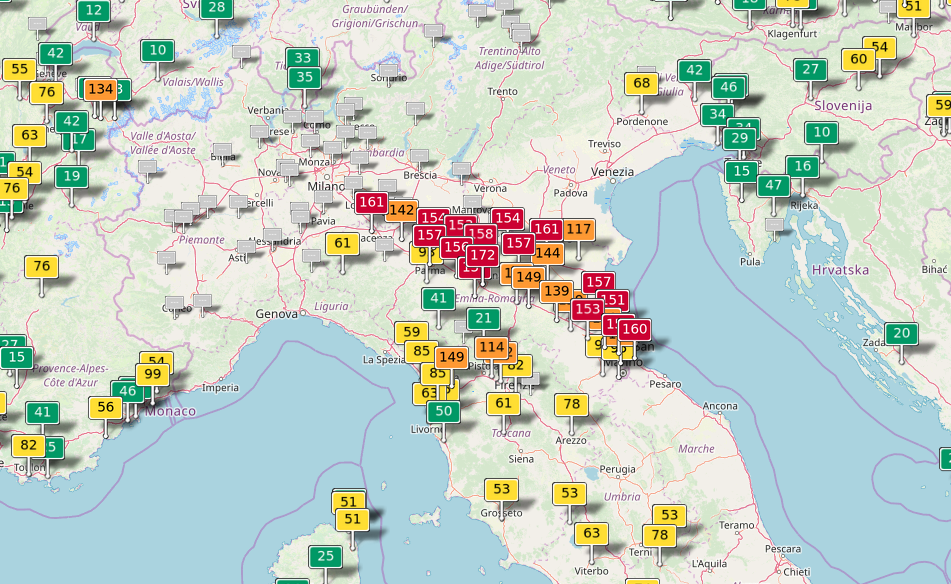
\includegraphics[width=25cm,height=10cm,keepaspectratio]{img/aqicn.png}
  \caption{acqin.org Labeled mapchart with the index of air pollution(the more polluted, the more the label is coloured red)}
  \label{fig:boat3}
\end{figure}
\subsubsection{waqi.org}
In this second app we have more types of data representation than before. We have a close-up on a specific location with the data relative to it represented in various formats!
\begin{figure}[H]
  \centering
  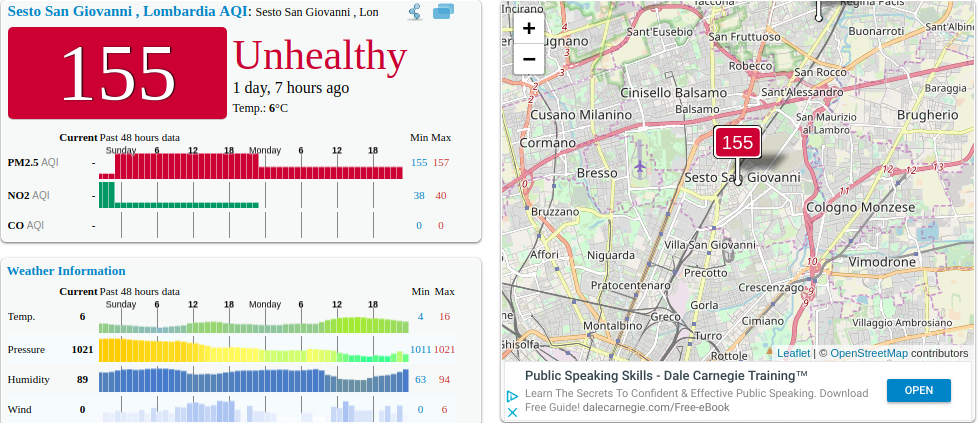
\includegraphics[width=15cm,height=10cm,keepaspectratio]{img/TechnicalExample.png}
  \caption{waqi.org in a example postion, which enhance the quality and quantity of data displayed}
  \label{fig:boat3}
\end{figure}

\end{itemize} 
\section{Proposal}
The solution provided will present the following representation. 
\subsection{Individual}
\subsubsection{Requirements}
We define here the requirements for the personal interfaces we decided to implement.
The smartphone app we were going to design must fulfill some requisites:
\begin{enumerate}
	\item Summarize all the information in an easy-to-use tool.
	\item Provide readable data about the behavior of a certain variable in time.
	\item Allow the most curious users to confront data between the/some stations.
\end{enumerate}
Build such a thing is not an easy task, given that the space is small and has to be optimized in order to display in the best quality possible those data.

The smartwatch app cannot be as full of details as the smatphone's, given the more restricted space, it will only visualize the last measurements and a daily basis.
\subsubsection{Reasoning about the dataset}
Given the variables the station is measuring and what has to be shown through the interfaces, we have defined a simple hierarchy of the information.
We decided to divide them in two groups:
\begin{description}
\item Variables strongly dependent on location, and immutable/less important data
	\begin{itemize}	
	\item Weather
	\item Hour, season
	\item Wind direction
	\item Location features
	\end{itemize}
	
\item Important variables, more likely to be studied and with some kind of behaviour
	\begin{itemize}
	\item CO2 ppm
	\item Wind speed
	\item Luminosity
	\item Temperature
	\item Umidity
	\item Rain
	\item Pressure
	\end{itemize}
\end{description}

\subsubsection{Smartphone Proposal}
The solution provided has to take into consideration that it has to give an easy representation of complex data. It is divided in two macroparts, a summary of the station first-group data and a view in detail of the most important variables.
The station is automatically selected if a notification(that will be sent if the smartphone is near a station) or a not at the open in the app is pressed, otherwise it will be chosen by the user through a map.


\begin{figure}[H]
  \centering
  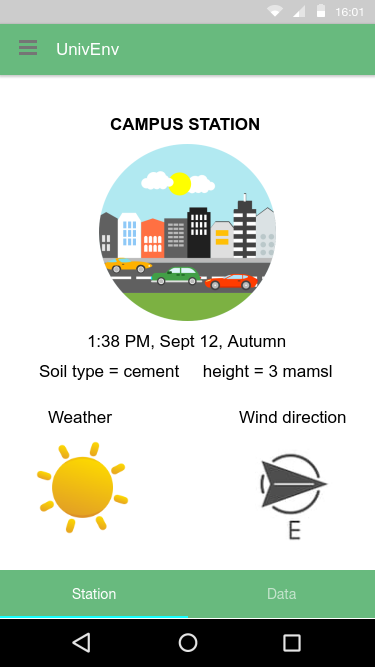
\includegraphics[width=4cm,height=10cm,keepaspectratio]{img/station.png}
  \hspace{0.1\textwidth}
  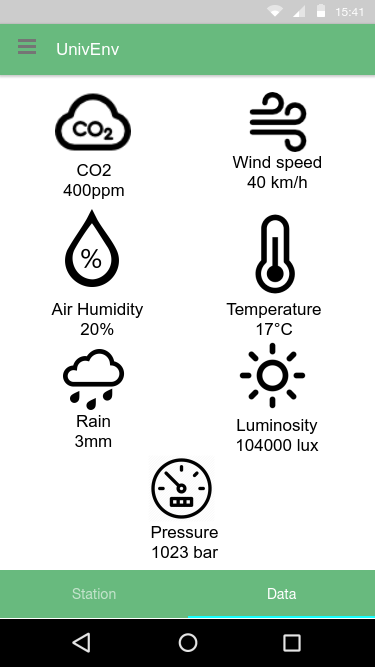
\includegraphics[width=4cm,height=10cm,keepaspectratio]{img/data.png}
  \hfill
  \caption{Smartphone activity}
  \label{fig:boat1}
\end{figure}

\subsubsection{User interaction}
INVISION LINK: https://invis.io/M5PI3T9Z3JX.

At the opening of the app, there are three possible scenarios:
\begin{enumerate}
    \item The user is not in the proximity of a eco station, so a map will be visualized with the nearest ecostation(1-2 km range) and the user will choose what station visualize.
    \item The user is near a station, presses the notification, the app will open up and the measurements of that particular station.
    \item The user is near a station, opens the app in the standard way and a popup will show up(You are near to "Vega ecostation", connect to it?).
  \begin{figure}[H]
  \centering
  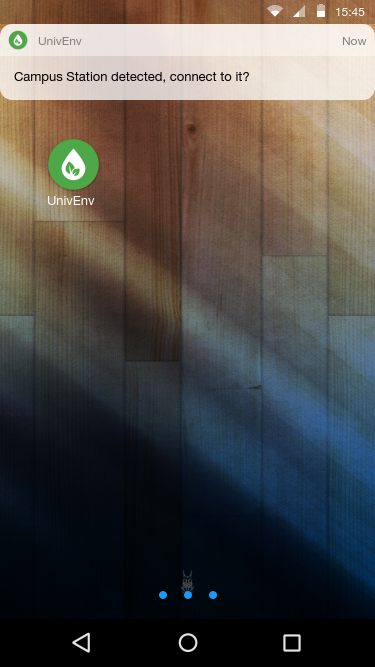
\includegraphics[width=4cm,height=10cm,keepaspectratio]{img/notismart.png}
  \caption{Smartphone notification}
  \label{fig:boat1}
\end{figure}
\end{enumerate}


When a station is selected, a general display of that station will be visualized, which contains:
\begin{itemize}
\item Station name
\item Time and season
\item Weather around that particular station
\item Type of soil and enviroment
\item Height in maslm
\end{itemize}

If the user presses the data tab, the icons of the most important variables will show up, with their current lecture already visible.

When an icon is pressed, the activity of that certain variable will popup up, in which the user can see how the last lecture approaches the annual max measure of that particular variable, as well as the behaviour of that variable in time(daily, monthly or yearly).

If the "Comparison" button is pressed, another activity will show up, which presents the comparison of actual lectures of the nearest stations and their behaviour in a week timespan.
In any moment, the user can use the Hamburger icon menu, which permit an easy navigation and simplify the return to the home screen, instead of force the user to a reetitive back arrow press.
  
\begin{figure}[H]
  \centering
  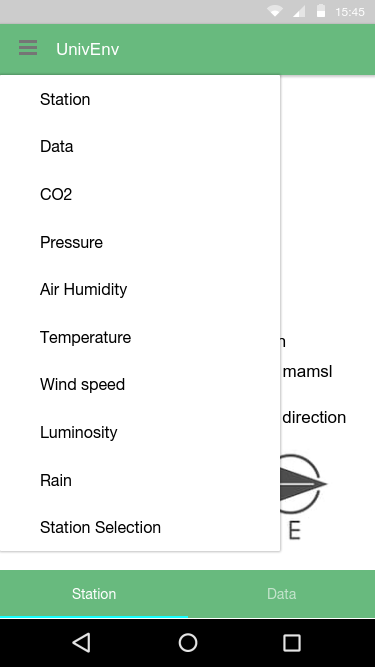
\includegraphics[width=4cm,height=10cm,keepaspectratio]{img/menu.png}  
  \caption{Hamburger menu}
  \label{fig:boat1}
\end{figure}
\subsubsection{Graphs used}
\begin{itemize}
\item \textbf{Map Chart}

This will permit at a user which is not at beacon-range distance to a station to choose a station within a 2 km range max. 

\item \textbf{Gauge chart}

It gives a representation to the max value registered in the season.

\item \textbf{Histogram chart}

We use this to show the history of a variable with different time ranges and an easy confrontation of last measure by different stations.

\item \textbf{Line chart}

It confront the lectures of the different station within a week time span.
\end{itemize}



\subsubsection{Smartwatch}
\begin{figure}[H]
  \centering
  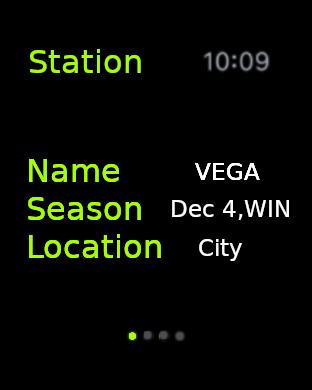
\includegraphics[width=4cm,height=10cm,keepaspectratio]{img/STATIONAW.png}
  \hspace{0.05\textwidth}
  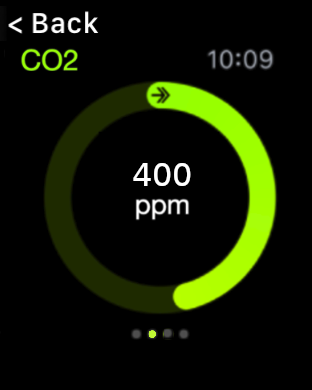
\includegraphics[width=4cm,height=10cm,keepaspectratio]{img/CO2AW.png}
  \hspace{0.05\textwidth}
  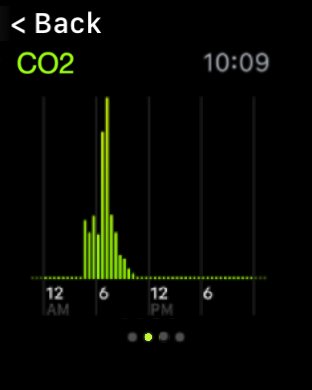
\includegraphics[width=4cm,height=10cm,keepaspectratio]{img/histoAW.png}
  \hfill
  \caption{An overview of the navigation pages}
  \label{fig:boat1}
\end{figure}
INVISION link: https://invis.io/6HPIZVO7FNE.

For the smartwatch, we based the design choices over \cite{apple}, in order to have to be as precise as possible.
Given, which is a simple device, we decided not to provide lots of data or difficult plots that might result not clear to the user.
We represent only the most important variables, with a little overview of the location of the station, as it's seen in the picture.

The general design of the application is \textbf{Glanceable}, with a \textbf{Modular Large Complication} placed in the smartwatch home screen.
The \textit{Gestures} we decided to introduce in the app are \textbf{Tap} and textbf{Horizontal swipe}.

The navigation of the app will be a \textit{Page-Based one}, with a total of 7 pages (one for each important variable plus 1 for station overview).
Like the smartphone, a notification in case a particular station is in range would be received by the smartwatch.

At the open of the app, a \textbf{Action Sheet} will pop up, letting the user choose over the different stations.After having choose a station, the app will open up like in Figure 7.
In any time, by pressing the \textbf{Back} button, the user can go back to the initial screen and can select another station.

\begin{figure}[H]
 \centering
  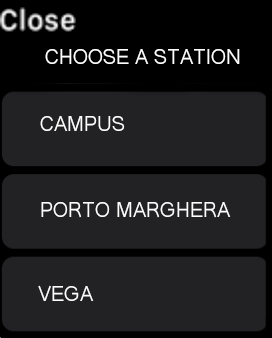
\includegraphics[width=4cm,height=10cm,keepaspectratio]{img/StationActionSheet.png}
  \hspace{0.05\textwidth}
  \hfill
  \caption{Action Sheet for station selection}
  \label{fig:boat1}
\end{figure}
The user can swipe through the pages, and in a page representing a variable, a double tap on 
the radar chart can change the type of data representation the page will visualize.

\subsubsection{Graphs used}
\begin{itemize}
\item \textbf{Radial bar chart}

We use it to visualize the current variable measurement with respect to a daily/montly/annual max value
\item \textbf{Histogram chart}

Is a simple plot that can give a quick view to a short history of the variables, in order to extract possible behaviors of a certain variable.
\end{itemize}

\begin{figure}[H]
  \centering
  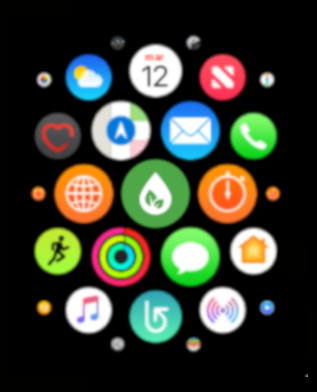
\includegraphics[width=4cm,height=10cm,keepaspectratio]{img/MenuHome.png}
  \hspace{0.05\textwidth}
  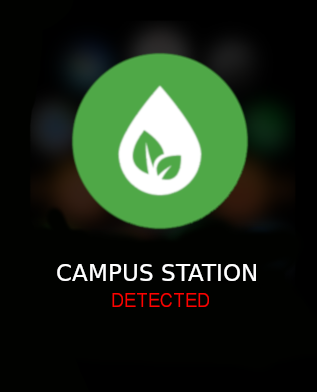
\includegraphics[width=4cm,height=10cm,keepaspectratio]{img/Notification.png}
  \hfill
  \caption{Notification and app menu design}
  \label{fig:boat1}
\end{figure}
\subsection{Public}
The public interface has been structured in two parts. 
\begin{itemize}
\item The first screen (Figure 2), is an image that represent the current state of our  environment depending on the variables defined before. If, for example, the level of CO2 is over the average level, we'll add some smog clouds in our representation. Now we define, for each variable, what we are going to add if the level is over the normal level. The temperature is given by a string in the upper-right part.
\begin{itemize}
\item CO2: smog clouds.
\item Air Humidity: fog.
\item Luminosity: bigger sun.
\item Wind speed and direction: wind icon and clouds.
\item Location (also height, type of soil, type of surrounding environment): is described by the image.
\item Time (hour/season): there is a string indicating what time is it. For the season, it's described by the image.
\item Pressure: arrows going down
\item Rain: clouds with rain
\end{itemize} 

This representation is thought to be as abstract as possible, in order to be accessible to all people (e.i. kids, adults, etc).
There'll be a sound output that will tell you what you are clicking, for helping blind people.

\begin{figure}[H]
  \centering
  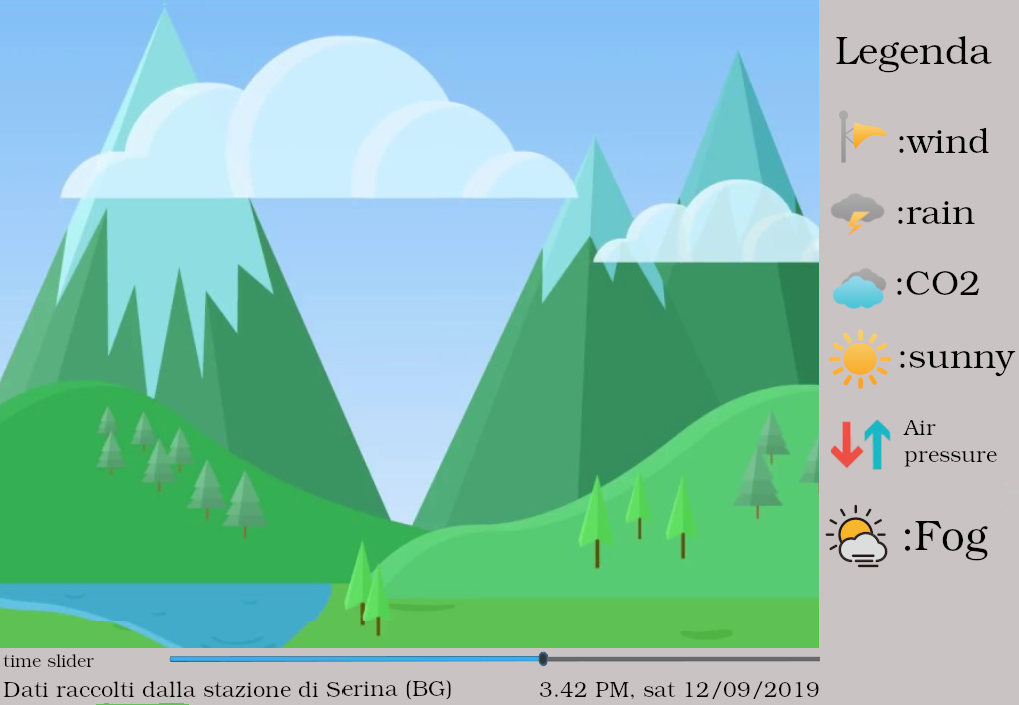
\includegraphics[width=0.7\textwidth]{img/default.png}
  \caption{Public interface}
  \label{fig:boat1}
\end{figure}

This is the main screen that welcomes an user approcing the Ambient display.
With a glance, the user will have some raw information about the data gathered by the nearest station.

\begin{figure}[H]
  \centering
  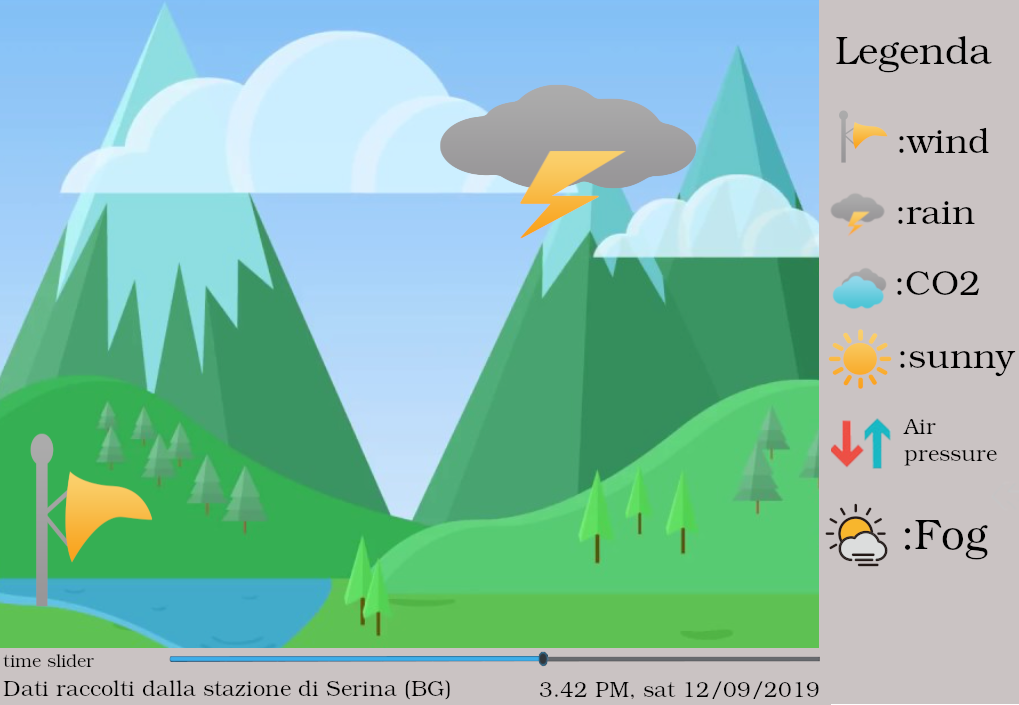
\includegraphics[width=0.6\textwidth]{img/wind+rain.png}
  \caption{Public interface with rain and wind}
  \label{fig:boat1}
\end{figure}

If there are some parameters that are out of the normal values the system will add graphical artifact to
inform the user (in our case we have abnormal values of CO2 and it's raining).
In the homescreen there is also a time slider that allows the user to view data from the past month. 
This is enable him to quickly compare the data gathetered from the station in few seconds.
 
\begin{figure}[H]
  \centering
  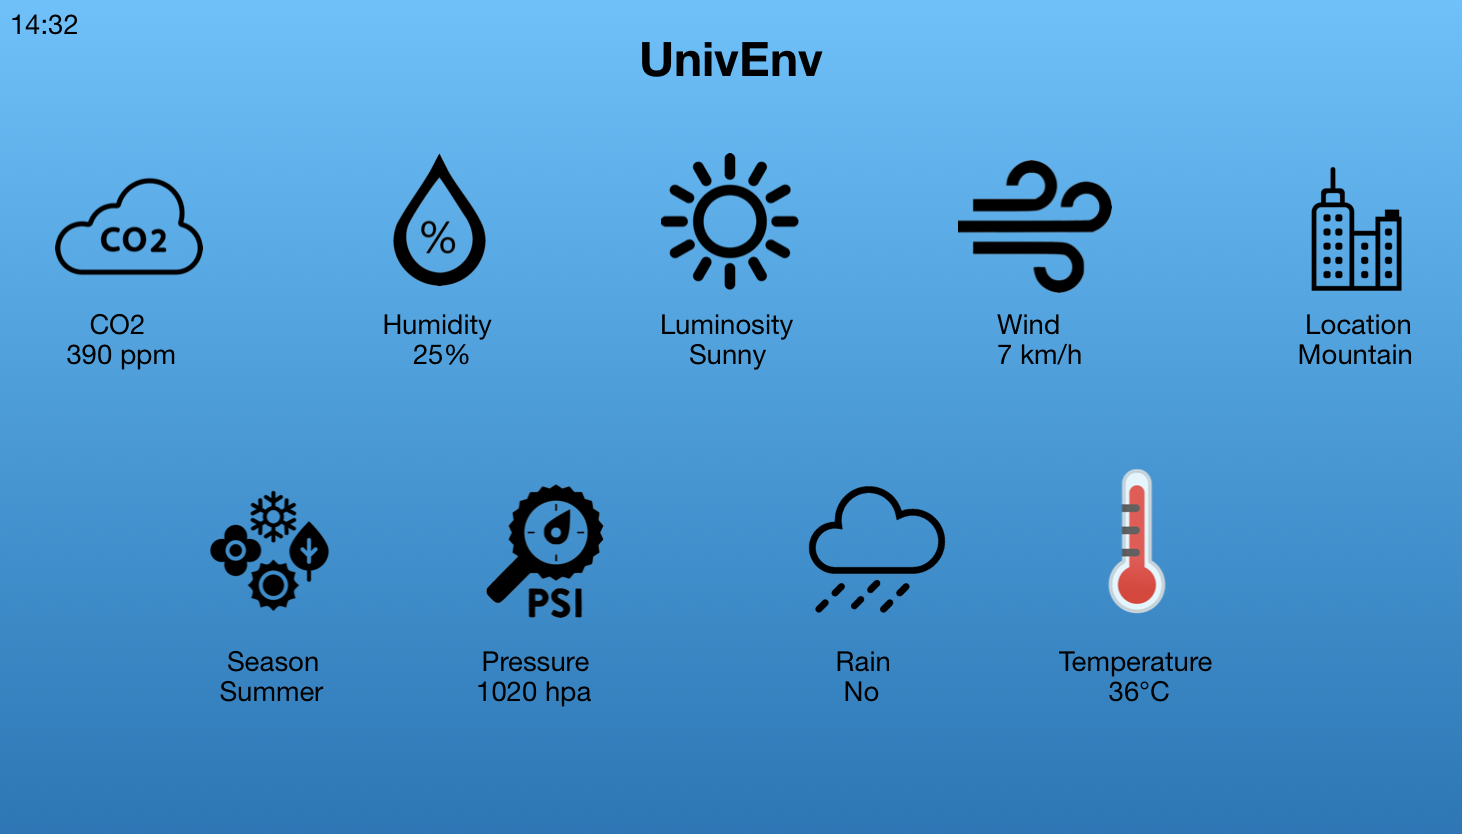
\includegraphics[width=0.6\textwidth]{img/p2.png}
  \caption{Info of public interface}
  \label{fig:boat2}
\end{figure}

The detailed view accessible touching the homescreen allows the user to see the raw data of the local station.
This give a detailed view of the surrounding in a short amount of time.
\end{itemize}
\newpage
\subsection{Technical}
OUR INITIAL MOCKUP INVISION link: https://invis.io/3WPJB0OEYAP.
This type of representation is for people that analyze the row data, so it has been chosen to use representations that maybe are less intuitive to understand but are more accurate. 
 It has also been introduced the comparison, which allows to select the type of data to compare, and compare it.
The system is divided in the following parts: 
\begin{itemize}
\item Login
\item Choice of the station
\item Overview and data representation of a single station  
\item Comparison
\end{itemize}
It has been chosen the following type of representation: 
\begin{itemize}
\item Weather Map
\item Radar chart
\item Line chart
\item Violin Plot
\item Scatterplot Matrix
\item Bar Chart
\item Parallel Plot
\end{itemize}
\subsection{User Interaction}
The technical application will be used by academic and technician to visualize and manipulate data in a more detailed way. The first screen that we are going to see in the technical app is the \textit{login screen} needed to authenticate the users with the permissions to visualize the data.

After the authentication we will have to select the station we want to display(In our example every station selected brings you to Porto Marghera station).
The overview of the selected station will then open up, with a comfortable menu on the left side with:
\begin{itemize}
	\item \textbf{Overview}, which summarize the overall situation in the current station.
	\item \textbf{Single station charts} with a lot of useful data representation, in order to better inspect the situation in the selected station
	\item \textbf{Comparision charts}, which permits to compare data between different stations
	\item \textbf{Change station} that lets the user change the focus on another station 
\end{itemize}
We used a fake user called Giuseppe Rossi with password 'admin', but even empty values will let you enter.
The only station we actually introduced are Serina and Porto Marghera, the other ones are placed only as mock data.
The user can change station(only between Porto Marghera and Serina) by pressing the \textbf{Change Station} label.

We have introduced some functionality in order to show how the complete and full working site will look like.
In any time, clicking on the name of the web application, the user can go back to the beginning(the choice of the station).
Many charts we used are interactive, that means that on action like mouse over the user will be show additional information for the data represented on the plot.

For example, if we select some elements they are highlighted, while in some chart like the violin, bar and line chart selecting a particular subset of measures the plot will be zoomed, a double click will remove the zoom.

\subsubsection{Single station charts}
Here the user can look at the charts we decided were optimal to show the historical behaviour and the distribution over a day of the different variables and the possible relations between a subgroup of the  variables.

We handled the selection of the variables with a combobox while the measurements showed in the	\textbf{Scatterplot Matrix} are handled with a series of checkboxes.

\subsubsection{Comparison charts}
In this section the user selects which station to compare with the checkboxes under every chart, by default the nearest two are automatically selected to be compared.
The \textbf{Parallel plot} can represent different variables of different stations, so it's layout will be controlled by a series of checkboxes(mocked).
Every time a station is selected to be compared, its name will show up on the left menu, and under those name the user can return to the overview of one of the nearest three stations.     

\subsection{Type of graphs}
It has been chosen those type of representation because they represent accurately the raw data. The exceptions are the radar chart, it has been chosen because it sum up all the variables(the values goes from 0 to 10, which represent the quality of that variable); and the Bubble map which represent the situation in that moment on the map.

\subsubsection{Weather Map}
We use this to put on a geographical view all the station, the user will select the particular station he wants to inspect the measurements
\begin{figure}[H]
  \centering
  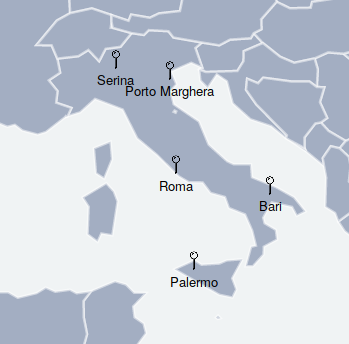
\includegraphics[width=0.7\textwidth]{img/WeatherMap.png}
  \caption{WeatherMap}
  \label{fig:rdrChart}
\end{figure}

\newpage

\subsubsection{Radar Chart}
The radar graph is a graphic method to represent set of datas consisting of multiple variables, representing them on axis with the same origin.
\begin{figure}[H]
  \centering
  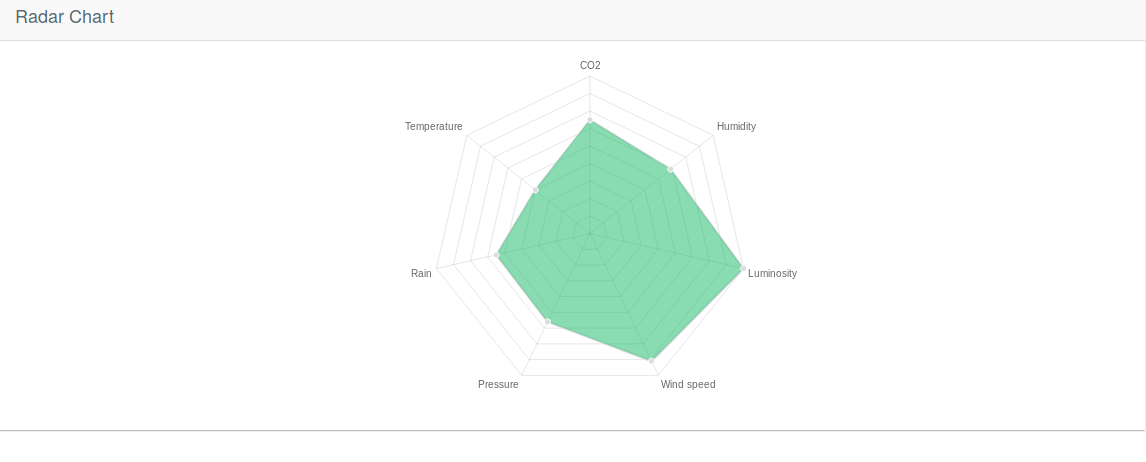
\includegraphics[width=0.7\textwidth]{img/RadarChart.png}
  \caption{Radar chart}
  \label{fig:rdrChart}
\end{figure}
This chart is used in our project to quickly check the optimality of the various parameters of a given building in the moment of the visualization.
with this tool we will be able to know which are the worst/best parameters with a glance and use this information to pick the right countermeasures.

\newpage

\subsubsection{Line Chart}
The line chart is a chart which displays a series of data points called "markers" connected by straight line segments.
\begin{figure}[H]
  \centering
  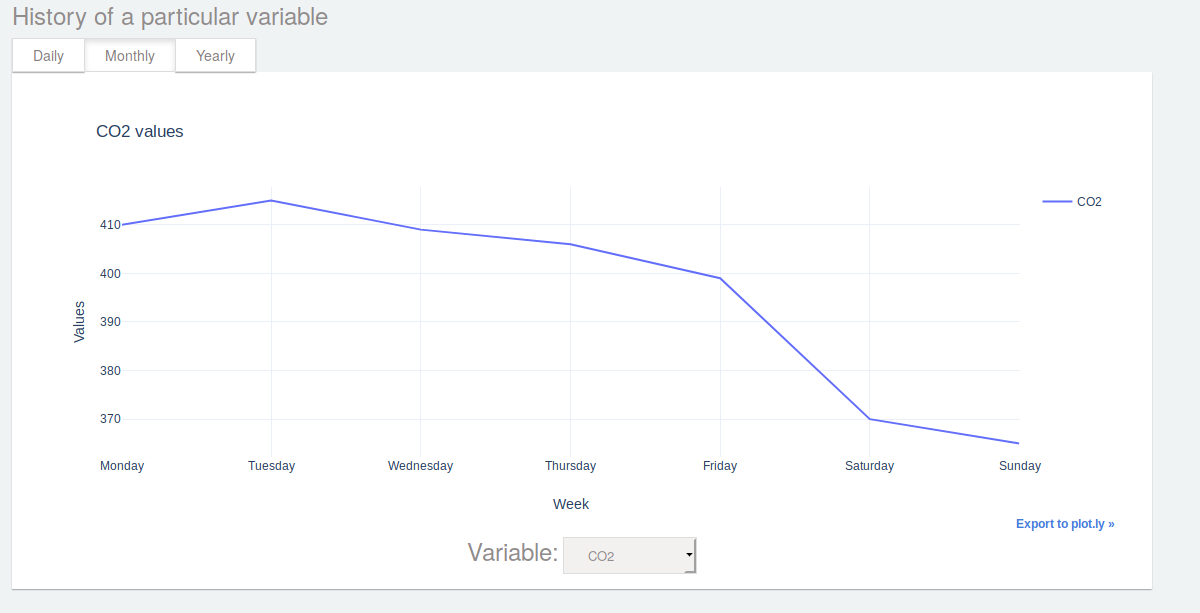
\includegraphics[width=0.9\textwidth]{img/LineChart.png}
  \caption{Line Chart}
  \label{fig:lnChart}
\end{figure}
We use this type of representation in our technical interface to display a single data over time, allowing us to appreciate its mutations in a certain period(daily, montly or yearly).

\newpage

\subsubsection{Violin plot}
A violin plot is a method of plotting numeric data. It is similar to a box plot but it is composed by four layers: The outer shape represents all possible results, with thickness indicating how common. The next layer inside represents the values that occur 95 percent of the time. The next layer (if it exists) inside represents the values that occur 50 percent of the time. The central dot represents the median average value. 
\begin{figure}[H]
  \centering
  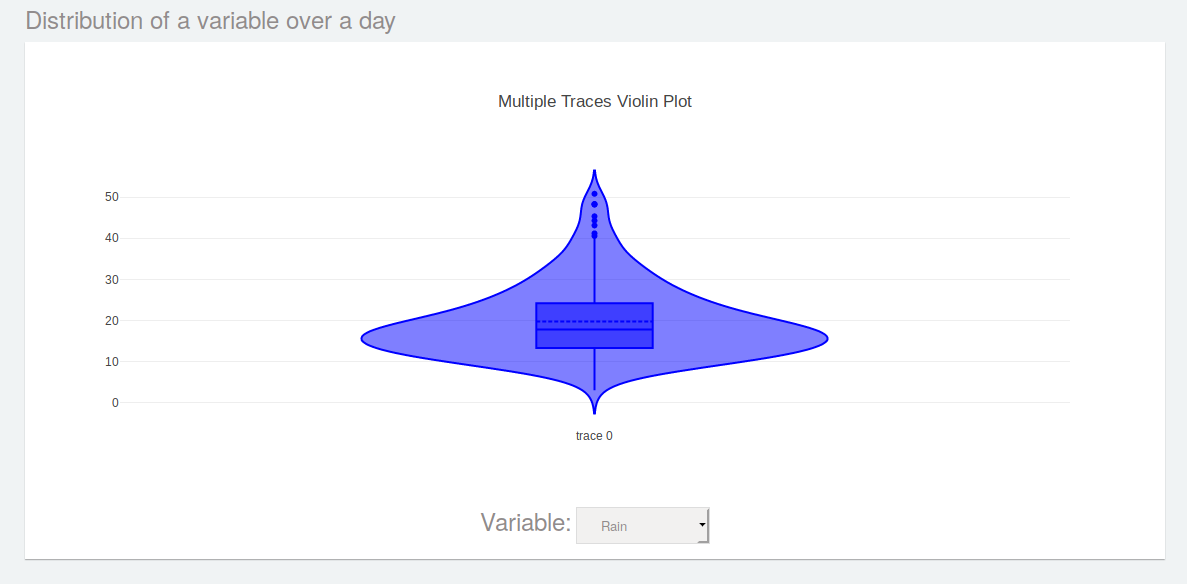
\includegraphics[width=0.9\textwidth]{img/ViolinChart.png}
  \caption{Violin Chart}
  \label{fig:scttrPlot}
\end{figure}

\newpage
\subsubsection{Scatterplot Matrix}
Scatterplot matrix is a particular type of graphs which combines different Scatterplot.
We use it to compare different variables of a single station, in order to discover relations between some enviromental specs
\begin{figure}[H]
  \centering
  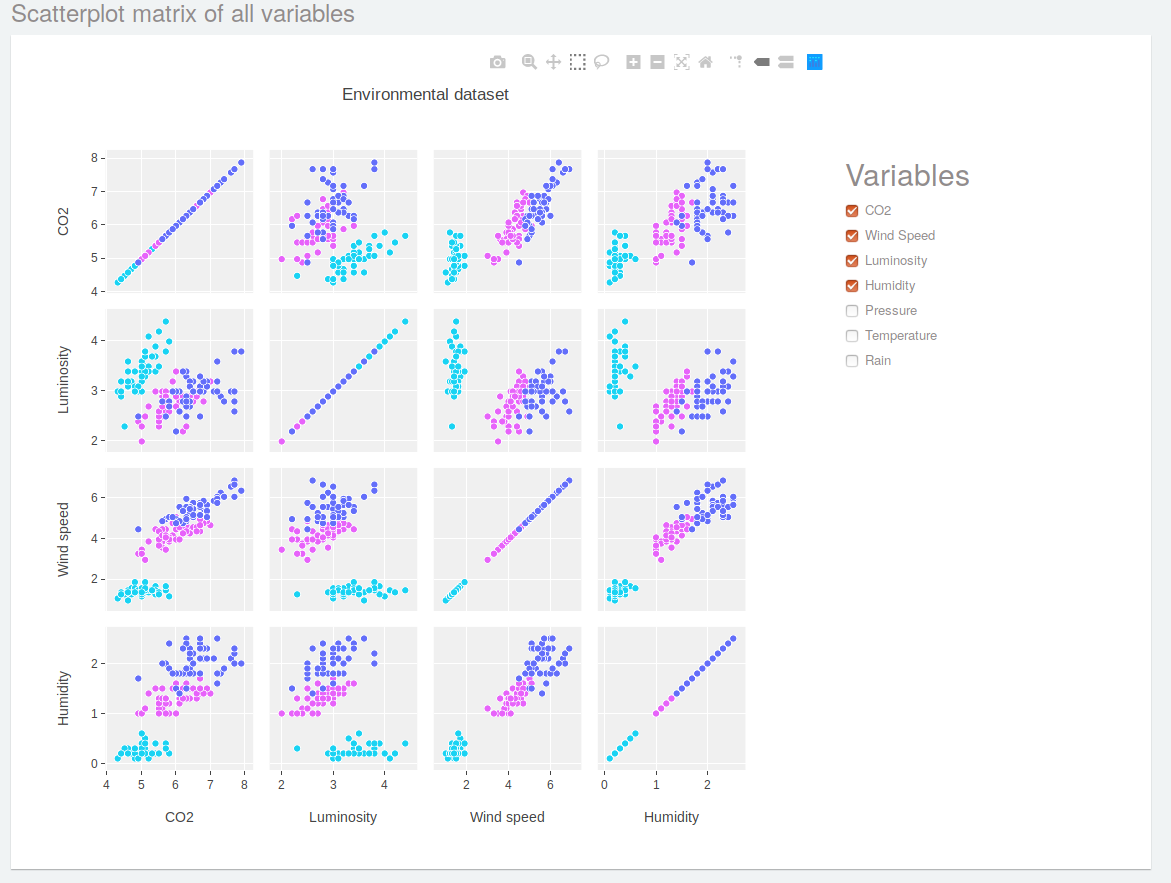
\includegraphics[width=0.9\textwidth]{img/ScatterplotMatrix.png}
  \caption{Scatterplot Matrix}
  \label{fig:scttrPlot}
\end{figure}
In our case we select with a series of checkbox which variable to display.
\newpage
\subsubsection{Bar chart}
The bar chart is used in the comparision between different station, for the last measurements of a particular variable.
This will give us a first hint on possible patterns, compare for example the different concentration of CO2 between an industrial area and a near mountain enviroment, or maybe the different level of humidity between two different type of soil.
We can choose which of the variables we want to show up.
\begin{figure}[H]
  \centering
  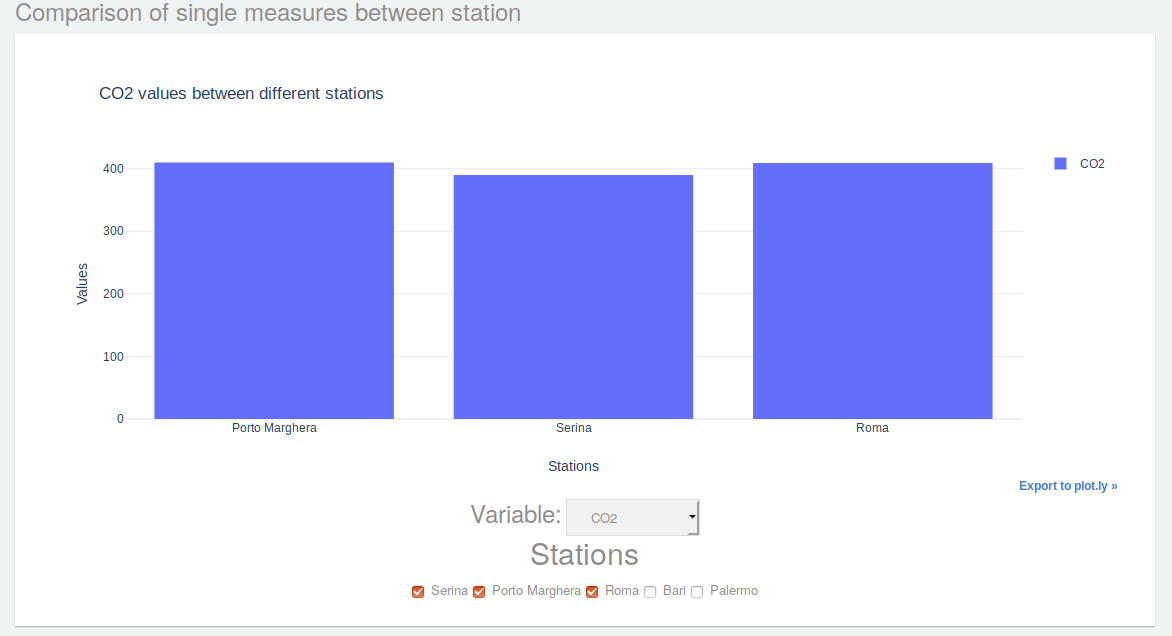
\includegraphics[width=0.9\textwidth]{img/BarChart.png}
  \caption{Bar Chart}
  \label{fig:scttrPlot}
\end{figure} 

\newpage

\subsubsection{Parallel Plot}
We used this particular graph in order to show possible hidden relations between other station measurements of the variables.
The closer the station are between them, the data might be influenced by the same enviromental condition, and might have some relation with one another, between station not so close there might be some relation of atmosferical and weather variables(maybe low-pressure conditions or perturbation).
\begin{figure}[H]
  \centering
  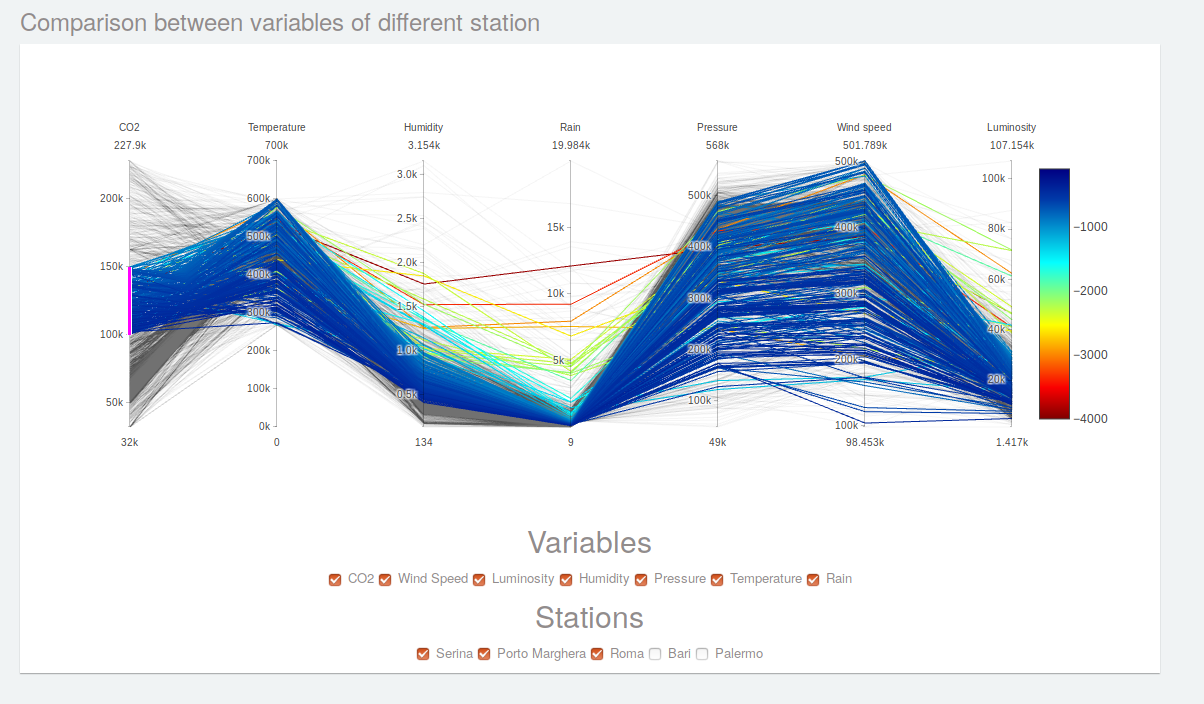
\includegraphics[width=0.9\textwidth]{img/ParallelPlot.png}
  \caption{Parallel Plot}
  \label{fig:scttrPlot}
\end{figure}






\newpage
%----------------------------------------------------------------------------------------
%	BIBLIOGRAPHY
%----------------------------------------------------------------------------------------
\section{Bibliography}
\begin{thebibliography}{99} % Bibliography - this is intentionally simple in this template

\bibitem B. E. Medlyn, C. V. M. Barton, M. S. J. Broadmeadow, R. Ceulemans{art}
Stomatal Conductance of Forest Species after Long-Term Exposure to Elevated CO2 Concentration: A Synthesis;
\newblock {The New Phytologist, vol. 149, n. 2, Feb. 2001.},  pp. 247-264.

\bibitem {apple}
Apple,\\ Human Interface Guidelines, Gestures; \\
\newblock {https://developer.apple.com/design/human-interface-guidelines/watchos/user-interaction/gestures/}

 
\end{thebibliography}

%----------------------------------------------------------------------------------------

\end{document}